\documentclass[12pt,a4paper]{article}
\renewcommand{\baselinestretch}{1.05}
\usepackage[spanish]{babel}
%\usepackage[utf8]{inputenc}

\usepackage{amsmath,amsthm,verbatim,amssymb,amsfonts,amscd, graphicx}
\usepackage{caption}
\usepackage{subcaption}
\usepackage{pgfplots}
\usepackage{booktabs}
\usepackage{float}
\usepackage{enumitem}
\usepackage{hyperref}
\usepackage[style=numeric,backend=biber]{biblatex}
\bibliography{bibliografia}

%Uso de la fuente Source Sans Pro

\usepackage[default]{sourcesanspro}
%\usepackage[T1]{fontenc}

%Controlar la partición de palabras.
\pretolerance=5000
\tolerance=6000

%Simbolo de euro
\usepackage{eurosym} % para el euro


%Definición de monospace para codigo inline y paquete listings para código fuente.
\def\code#1{\texttt{#1}}
\usepackage{listingsutf8}
\lstset{
    %extendedchars=false,
    %inputencoding=utf8
}
\usepackage{color}
\definecolor{grisclarito}{gray}{0.95}

\lstdefinestyle{customc}{
  %belowcaptionskip=1\baselineskip,
  breaklines=true,
  frame=single,
  %xleftmargin=\parindent,
  language=Python,
  showstringspaces=false,
  %basicstyle=\ttfamily,
  keywordstyle=\bfseries\color{green!40!black},
  commentstyle=\itshape\color{purple!40!black},
  identifierstyle=\color{blue},
  stringstyle=\color{orange},
  backgroundcolor=\color{grisclarito}
}

\lstdefinestyle{customhtml}{
  %belowcaptionskip=1\baselineskip,
  breaklines=true,
  frame=single,
  %xleftmargin=\parindent,
  language=HTML,
  showstringspaces=false,
  %basicstyle=\ttfamily,
  keywordstyle=\bfseries\color{green!40!black},
  commentstyle=\itshape\color{purple!40!black},
  identifierstyle=\color{blue},
  stringstyle=\color{orange},
  backgroundcolor=\color{grisclarito}
}

\hypersetup{
  colorlinks=true,
  linkcolor=black,
  urlcolor=blue
}

%\setlength{\parindent}{0pt}
\topmargin0.0cm
\headheight0.0cm
\headsep0.0cm
\oddsidemargin0.0cm
\textheight23.0cm
\textwidth16.5cm
\footskip1.0cm

\renewcommand*\contentsname{Índice}
\newcommand{\mylabel}[2]{#2\def\@currentlabel{#2}\label{#1}}

\usepackage{graphicx}
\begin{document}
\begin{titlepage}
  \centering
  
\includegraphics[width=0.6\textwidth]{imagenes/ugr.png}\par\vspace{1cm}
  {\scshape\large Fundamentos de Redes \par} \vspace{1cm}
  {\huge\bfseries Comunicación bidireccional en arquitecturas cliente/servidor \par}
  \vspace{0.4cm}
  {\large\itshape El protocolo \textbf{WebSocket}\\}
  \vspace{0.6cm}
  {\large\itshape  Juan Francisco Díaz Moreno \\ Javier Sáez de la Coba \par} \vspace{1.00cm}
  Curso 2018-2019 \\
  \vfill

  % Bottom of the page
  {\large \today\par}
\end{titlepage}

\tableofcontents
\newpage

\setlength{\parskip}{10pt}

\section{Introducción}

% Hablar sobre la necesidad de una comunicación servidor -> cliente.

El modelo Cliente/Servidor es la tecnología que proporciona al usuario final el acceso transparente a las aplicaciones, datos, servicios o cualquier recurso de un servidor.

El cliente es el que inicia un requerimiento de servicio. Administran la interfaz de usuario, procesan la lógica de la aplicación, recibe los resultados y les da formato.

El servidor es la entidad que provee un servicio y devuelve resultados; ejecuta el procesamiento de datos, aplicaciones y manejo de la información o recursos. Es reactivo, pues realiza una función posterior a una petición o a la ejecución de una transacción requerida por el cliente u otro servidor.

¿Que ocurriría si necesitáramos que el servidor dejara de ser un elemento reactivo y tomara un papel activo en la comunicación y pudiera enviar datos cuando quiera al cliente sin tener que esperarlo?

\section{Evolución histórica}

% Como se ha ido abordando el tema de servidor->cliente a lo largo del tiempo. Poner alguna línea de tiempo.



Vamos a comenzar resumiendo las técnicas de comunicación bidireccional que existían antes de la llegada de los WebSockets. 

Internet no comenzó preparado para ser tan dinámico, si no para ser una colección de documentos HTML conectados unos con otros mediante enlaces formando una red de información. Los clientes únicamente descargaban de los servidores Web las páginas HTML tal y como estaban guardadas en éstos. Los servicios tecnológicos evolucionaron permitiendo páginas dinámicas, es decir, páginas cuyo contenido se generaba para cada cliente conectado.

Aunque las páginas web fueran dinámicas usando scripting de lado del cliente con lenguajes como \emph{VBScript} o \emph{JavaScript} las páginas no podían recibir información del servidor más allá de la obtenida en la carga inicial. Si se querían obtener nuevos datos había que recargar la página completa.

Una evolución de estas páginas dinámicas fue el desarrollo de sitios web que imitaban la utilidad de aplicaciones de escritorio. Para evitar recargar la página completa, se dividía en marcos (\emph{iframes}) que contenían elementos de la aplicación. Estos marcos se recargaban de forma independiente y conseguían mostrar información actualizada, pero con el inconveniente de que esto solo ocurría cuando el cliente hacía una petición al servidor.

Estas técnicas arriba descritas solo nos muestran casos en los que el cliente pide datos nuevos al servidor, pero si el servidor tiene información nueva que dar al cliente no podía mandársela hasta que no hiciera una petición.

La primera aproximación a la solución de que el servidor mandara información al cliente era la técnica del \emph{HTTP Polling}. En ella el navegador automáticamente hacía peticiones al servidor de forma periódica en busca de nuevos datos. Esta técnica era muy ineficiente y bastante ineficaz. Esta técnica no es una comunicación real entre el servidor y el cliente, esto puede llevar a sobrecargas en la red y en el servidor debido a peticiones innecesarias por parte del cliente para intentar obtener datos nuevos cuando realmente no era necesario. 

Una solución a esta técnica pasó por usar plugins externos. Uno de ellos era LiveConnect. Con LiveConnect un applet escrito en Java se comunicaba con el servidor y pasaba la información a los scripts JavaScript que se ejecutaban en la página. Un problema grave de LiveConnect era que dependía de la versión exacta de la máquina virtual de Java integrada en el navegador, lo que llevaba a problemas de compatibilidad entre distintas plataformas. Debido a esto se popularizó la técnica del Forever Frame. Esta forma de comunicación servidor -> cliente aprovecha la extensión HTTP 1.1 y su opción de chunked encoding, donde los datos se mandan de forma troceada. Esto permitía abrir un iframe de fondo que pidiera al servidor información. El servidor lo mandaba los datos de forma troceada. A medida que iba llegando se iba cargando en el marco y un script en la página iba comprobando los datos contenidos por ese marco.

Con la llegada de AJAX (Asynchronous JavaScript And XML) las peticiones al servidor no tienen por qué ser iniciadas por el usuario. Desde el mismo código JavaScript de la página se inician peticiones al servidor. Esto posibilita las técnicas de Long-Polling, donde el código AJAX abre una conexión al servidor que se mantiene abierta. Cuando el servidor manda información la conexión se cierra y el cliente vuelve a abrirla a la espera de nuevos datos.

Con la llegada de HTML5 se introdujeron nuevos métodos de comunicación cliente-servidor. Uno de ellos son los SSE (Server-Sent Events). Mediante estos el servidor puede mandar mensajes de forma asíncrona al cliente. Sin embargo, el cliente tiene que hacer una petición POST normal para responder al servidor, haciendo así dos conexiones distintas. Con la llegada del protocolo WebSockets cliente y servidor mantienen una conexión única activa entre ellos por los que pueden mandar mensajes de forma bidireccional. Estos mensajes pueden ser tanto texto como datos binarios, permitiendo mandar no solo información textual (contenido texto de la página o scripts javascript) sino elementos multimedia como imágenes o vídeos entre otros.





\section{Presentación del protocolo WebSockets}

% Que es WebSockets, para que se utiliza, que navegadores lo soportan y que aplicaciones populares lo usan.

WebSocket es una tecnología que proporciona un canal de comunicación bidireccional y full-duplex sobre un único socket TCP. Está diseñada para ser implementada en navegadores y servidores web, pero puede utilizarse en cualquier aplicación cliente/servidor.

​Con esta API, puede enviar mensajes a un servidor y recibir respuestas controladas por eventos sin tener que consultar al servidor para una respuesta.

​Los WebSockets necesitan ser implementados tanto del lado del cliente como del servidor. En el primero, la API es una parte de HTML 5. En el lado del servidor necesitamos una librería que implemente WebSockets, aunque en la actualidad casi todos los servidores las soportan.

​En el lado del cliente, WebSocket está ya implementado en Mozilla Firefox 8, Google Chrome 4 y Safari 5, así como la versión móvil de Safari en el iOS 4.2 y en el Internet Explorer 10.

​Ejemplos de usos de WebSockets:
\begin{itemize}
\item Whatsapp Web.
\item Facebook
\item Netflix.
\item Twitch.
\item Bet365.
\item ShareLatex
\item GitHub
\end{itemize}


\section{Historia de WebSockets}

% Como surgió, quién lo hizo, gráfico de la implementación temporal del protocolo.
​WebSocket apareció por primera vez en la especificación de HTML5 referenciado como TCPConnection. Fue en junio de 2008 cuando una serie de debates llevados a cabo por Michael Carter resultaron en la primera versión del protocolo que se conocería como WebSocket.

​El nombre fue dado por Ian Hickson y Michael Carter, siendo el primero quien autorizó su inclusión en HTML5 y el segundo quien lo anunció en su blog.

​En Diciembre de 2009, Google Chrome 4 fue el primer navegador que lo implementó por completo. 

​Después de que el protocolo fuese implementado y permitido por diversos navegadores, el RFC fue publicado en diciembre de 2011, dando por finalizada la implementación de WebSocket.

Aquí mostramos una linea de tiempo de la implementación de WebSockets en los distintos navegadores.

\begin{figure}[H]
\centering
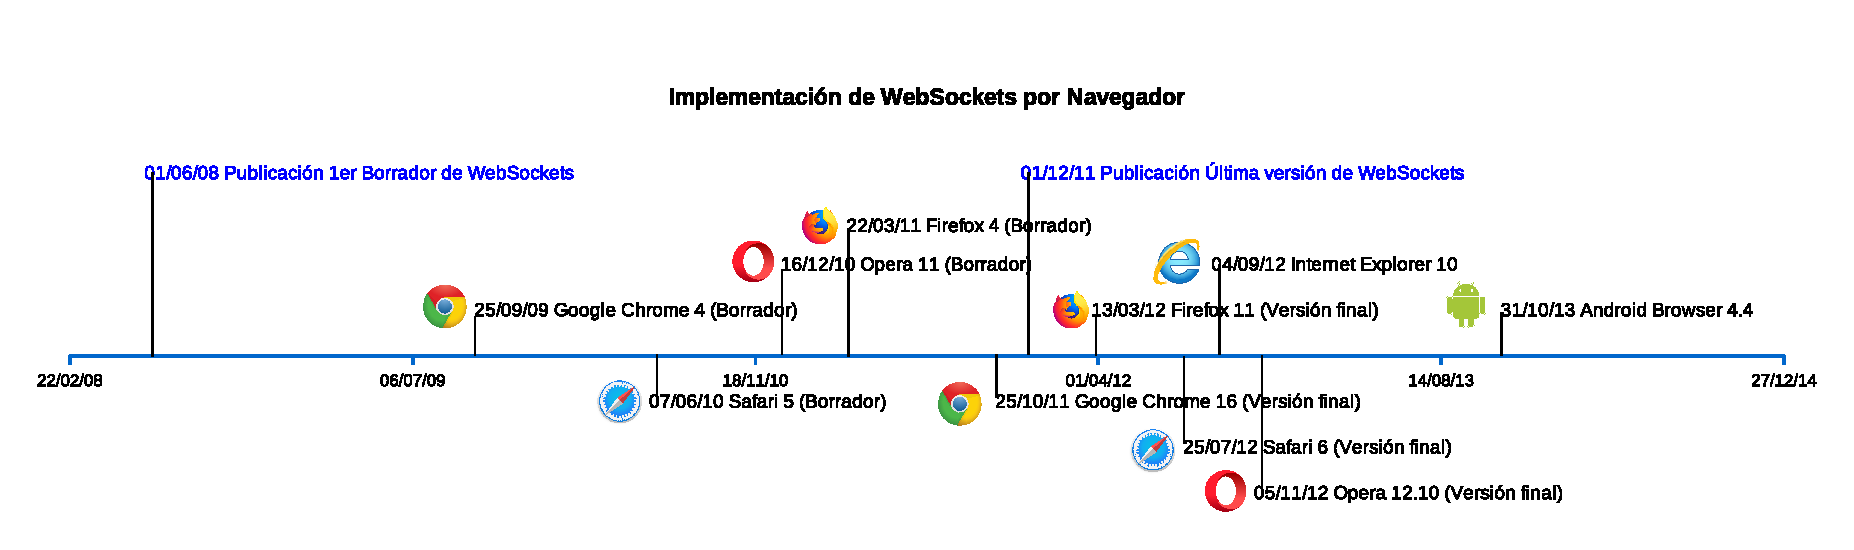
\includegraphics[scale=0.55]{imagenes/timeline.pdf}
\end{figure}

\section{Utilidad de WebSockets}

% Ventajas y desventajas. Lenguajes en los que está implementado. Ejemplos genéricos de usos.

WebSockets tiene una gran cantidad de ventajas entre las que destacan:
\begin{itemize}
\item Comunicación full-duplex entre cliente y servidor.
\item Mejora la eficiencia de la comunicación cliente-servidor, estableciendo una única conexión.
\item Estandariza las comunicaciones evitando soluciones propietarias.
\item API bien documentada y fácil de implementar e integrar en nuestras aplicaciones.
\item Permite crear aplicaciones modernas con requerimientos de comunicación en tiempo real.
	
\end{itemize}

WebSockets se implementa de lado de cliente en JavaScript pero necesita soporte de lado de servidor. Una gran cantidad de lenguajes de programación permiten el uso de WebSockets, permitiendo crear servidores de aplicaciones en el lenguaje que queramos. Un ejemplo de estos lenguajes que soportan WebSockets son: C, JavaScript, Python, Ruby, Haskell, Java, PHP, Objetive-C, Swift...

\section{Detalle técnico de una conversación servidor-cliente mediante WebSockets}

% Diagramas y explicación técnica de WebSockets. Advertir de el temaso con los proxys.

Ahora presentamos el esquema de comunicación usado para iniciar una conexión mediante WebSockets:

\begin{figure}[H]
\centering
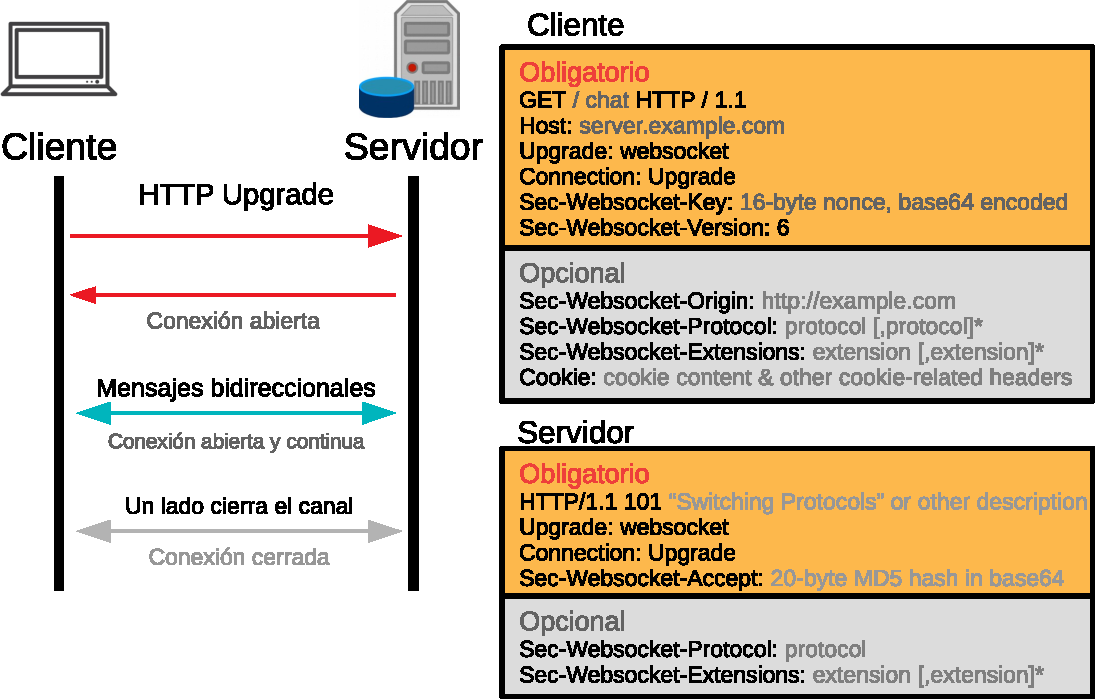
\includegraphics[scale=0.8]{imagenes/diagrama.pdf}
\end{figure}

En primer lugar, el cliente solicita conectarse a través de una llamada HTTP cuya cabecera sería la que vemos en la parte superior derecha. En ella distinguimos las partes más importantes:
\begin{itemize}
\item Host es el nombre del servidor al que estamos llamando.
\item Upgrade indica que es una llamada de actualización, en este caso WebSocket.
\item Conneccion define que es una llamada de actualización.
\item Sec-Websocket-Key es una clave generada aleatoriamente que es posteriormente usada para autentificar la respuesta.
\item Sec-Websocket-Origin muestra dónde se ha originado la petición. En el lado del servidor es usado para comprobar la autenticación de la petición.
\end{itemize}
Una vez que el servidor comprueba la autentificación, envía una respuesta que se ve como en la parte inferior derecha.
\begin{itemize}
\item Sec-Websocket-Accept tiene una clave que es decodificada y comparada con la key enviada para ver que la respuesta se está enviando al cliente correcto.
\end{itemize}
Una vez que la conexión está abierta, el cliente y el servidor pueden enviar los datos de uno a otro. Estos datos son enviados en forma de pequeños paquetes usando el protocolo TCP, por lo que no son visibles directamente dentro de la herramienta de desarrolladores.

Finalmente, tanto el cliente como el servidor pueden cerrar el canal de comunicaciones que comparten.

\section{Implementación de una app usando WebSockets}

% Implementación de una app simple usando websockets y análisis de la misma.

Vamos a implementar una app de prueba muy simple tipo chat para poder demostrar el funcionamiento de los WebSockets. Para ello vamos a utilizar SocketIO junto con Flask. SocketIO es una librería multilenguaje que se utiliza para establecer conexiones entre cliente y servidor de forma bidireccional. Entre las múltiples formas de conexión que tiene se encuentran WebSockets. SocketIO está implementado en gran variedad de lenguajes de programación: desde JavaScript hasta Scala. Nosotros vamos a usar la implementación en Python para el framework de desarrollo web Flask.

Empezamos instalando los paquetes necesarios:

\begin{lstlisting}
pip install flask-socketio eventlet
\end{lstlisting}

Ahora creamos las dos partes necesarias de nuestra aplicación: el código que se ejecuta en el cliente y el código que se ejecuta en el servidor. Para la parte del servidor usamos la facilidad de Flask para definir las rutas de nuestra aplicación.

\lstinputlisting[language=Python, firstline=7, lastline=40, style=customc]{demo/app_latex.py}

Vemos que se reduce a inicializar Flask y SocketIO y definir rutas y eventos a los que responder. con el decorador siguiente definimos la función que se encarga de procesar los mensajes que lleguen por el WebSocket del tipo \code{my-event}.
\begin{lstlisting}[style=customc]
@socketio.on('my_event', namespace='/test')
\end{lstlisting}

De forma muy similar implementamos en el lado del cliente (index.html) las conexiones pertinenentes de SocketIO esta vez en JavaScript.

\lstinputlisting[style=customhtml]{demo/templates/index_latex.html}

Aquí hacemos una cosa similar. Después de importar el código de SocketIO abrimos el socket que usará WebSockets contra el servidor y definimos las funciones que manejarán los mensajes recibidos a través del socket. Aquí se puede observar que la sintáxis de uso del WebSocket es muy similar en ambos lenguajes. Esto se debe a que la librería SocketIO estandariza bastante las funciones a usar.

El código de la aplicación anterior da lugar a la siguiente app:
\begin{figure}[H]
\centering
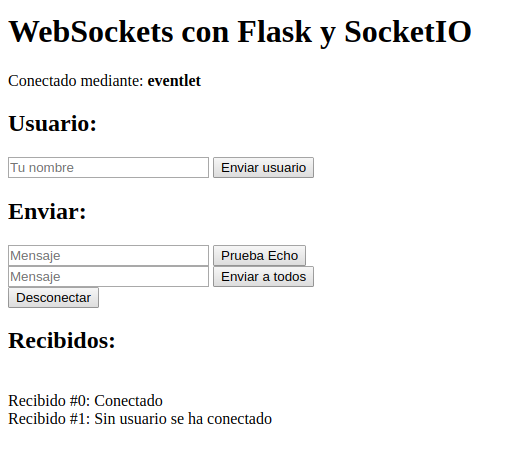
\includegraphics[scale=0.80]{imagenes/app.png}
\end{figure}

Todo el código así como este documento se encuentran en \url{https://github.com/jscoba/fr-websockets}


% \section{Bibliografía}
\nocite{*}
% Pegar en formato LaTeX el archivo de bibliografía que tenemos.
\printbibliography


\end{document}
